\documentclass[11pt,a4paper]{article}

\usepackage[margin=1in]{geometry}
% !TEX program = xelatex
\usepackage{fontspec}
\setmainfont{Figtree}[Path=fonts/,Extension=.ttf,UprightFont=*-Regular,BoldFont=*-Bold,ItalicFont=*-Italic,BoldItalicFont=*-BoldItalic]
\usepackage{enumitem}
\usepackage{hyperref}
\usepackage{parskip}
\usepackage{titlesec}
\usepackage{longtable}
\usepackage{array}
\usepackage{xcolor}
\usepackage{verbatim}
\usepackage{graphicx}
\graphicspath{{diagrams/}}
\newcommand{\flowbox}[2]{\fbox{\parbox[c]{#1}{\centering\small #2}}}

\setlist[itemize]{topsep=2pt,itemsep=2pt,parsep=0pt}
\setlist[enumerate]{topsep=2pt,itemsep=2pt,parsep=0pt}
\renewcommand{\arraystretch}{1.15}
\setlength{\tabcolsep}{4pt}

\titleformat{\section}{\large\bfseries}{}{0em}{}
\titleformat{\subsection}{\normalsize\bfseries}{}{0em}{}

\newcolumntype{L}[1]{>{\raggedright\arraybackslash}p{#1}}

\hypersetup{
    colorlinks=true,
    linkcolor=blue,
    urlcolor=blue
}

\setlength{\emergencystretch}{3em}










\begin{document}
\begin{center}
{\LARGE \textbf{Cogito Platform Release}}\\[4pt]
{\Large \textbf{Updated Release Scope}}\\[8pt]
{\normalsize Confirmed scope with content and design follow-ups}\\
{\normalsize Date: October 18, 2026}
\end{center}
\vspace{1em}


This revision incorporates FINAL SCOPE - Cogito Academy v3, received on October 12, and client follow-up answers received on October 13. It replaces earlier proposed prices and unresolved rules with v3 decisions. Activities now follows the confirmed Masterclasses/\allowbreak{}Cohorts/\allowbreak{}Other structure and app-style cards. Earlier follow-up questions are resolved. October 16 additions cover targeted landing-page improvements and branded report PDFs; remaining content/\allowbreak{}design dependencies are listed separately. All v3 numeric settings are admin-editable defaults unless stated otherwise.

\textbf{Payment boundary:} incoming student Marks purchases (packages and exact top-ups) remain through Midtrans, with gateway-confirmed crediting. KlikBCA Bisnis refers only to outgoing tutor/\allowbreak{}KOL payments made by admin outside the app. Admin records the actual transferred amount, date/\allowbreak{}reference and paid/\allowbreak{}settled status. No admin-verified direct-transfer top-up route, outgoing Midtrans payments, automated bank payouts or cash refunds are included.

\section*{1. Current application and release scope}

{\small
\begin{longtable}{|L{28.54mm}|L{52.57mm}|L{69.09mm}|}
\hline
\textbf{Area} & \textbf{Existing application} & \textbf{Changes in this iteration} \\ \hline
\endfirsthead
\hline
\textbf{Area} & \textbf{Existing application} & \textbf{Changes in this iteration} \\ \hline
\endhead
On-demand classes & Private/\allowbreak{}group bookings and 2-4-session series; existing payment/\allowbreak{}cancellation flow & Keep these class types and charging/\allowbreak{}cancellation rules. Replace pricing/\allowbreak{}tutor-fee calculations with the v3 rate card. \\ \hline
Economy and wallet & Packages, wallet/\allowbreak{}ledger and available/\allowbreak{}held balance foundation & New packages, exact top-up, admin economy page and cohort/\allowbreak{}masterclass holds with per-session deductions. Existing Marks remain untouched; all Marks never expire. \\ \hline
Big classes & No public cohort/\allowbreak{}masterclass seat enrollment & One shared model for cohorts and masterclasses; Classes page, curriculum, tutor assignment, seats, payment plans and returns. \\ \hline
Reports & Three-field session completion reports & Extend to all class types; 600 characters per field; reminders for incomplete reports; three-month student PDF export. No new attendance sheet or per-student notes. \\ \hline
Tutor payouts & Manual payment records/\allowbreak{}history/\allowbreak{}CSV; non-BCA transfer fee & Tax profiles/\allowbreak{}settings/\allowbreak{}override, session-linked payout history, immutable snapshots, void-with-note and monthly tax CSV. Bank transfers stay external. \\ \hline
Referrals & No referral campaigns/\allowbreak{}rewards identified in the reviewed baseline & Registration-only friend/\allowbreak{}KOL codes, welcome/\allowbreak{}reward ledger, semester caps, campaign settings, history and external settlement records. \\ \hline
Website/\allowbreak{}CMS & Sanity content sources and existing Activities/\allowbreak{}tutor pages & Merge Activities; migrate its source to app DB/\allowbreak{}API. Fix calendar agenda duplicates, remove landing Activities and Start Learning. Knowledge Bank/\allowbreak{}Calendar migration comes last. Website tutor lists read app profiles immediately, including an initial empty state. \\ \hline
\end{longtable}
}

Existing-state findings are from the previously reviewed source (cogito-app commit 14dc4486 and local cogito-acad checkout), not production verification.

\section*{2. Prices, exact top-up and admin economy}

\subsection*{Marks packages}

{\small
\begin{longtable}{|L{23.56mm}|L{41.23mm}|L{41.23mm}|L{41.23mm}|}
\hline
\textbf{Package} & \textbf{Marks} & \textbf{Rate per Mark} & \textbf{Price} \\ \hline
\endfirsthead
\hline
\textbf{Package} & \textbf{Marks} & \textbf{Rate per Mark} & \textbf{Price} \\ \hline
\endhead
Starter & 50 & Rp7.000 & Rp350.000 \\ \hline
Learner & 150 & Rp6.500 & Rp975.000 \\ \hline
Explorer & 250 & Rp6.000 & Rp1.500.000 \\ \hline
Pioneer & 500 & Rp5.500 & Rp2.750.000 \\ \hline
\end{longtable}
}

Existing wallet balances are unchanged. Purchased and bonus Marks share the same balance and spending rules; neither expires. IDR figures use Indonesian formatting.

\subsection*{Exact top-up: included}

Non-package amounts use the applicable package-tier rate plus Rp250/\allowbreak{}Mark: 1-149 = Rp7.250; 150-249 = Rp6.750; 250-499 = Rp6.250; 500+ = Rp5.750. Exact amounts 50/\allowbreak{}150/\allowbreak{}250/\allowbreak{}500 use package prices instead. If an exact top-up costs at least the next larger package, offer that package instead. Example: 140 Marks would cost Rp1.015.000, so offer 150 for Rp975.000. Other examples: 31 = Rp224.750; 176 = Rp1.188.000; 320 = Rp2.000.000; 600 = Rp3.450.000.

\subsection*{On-demand rate card}

{\small
\begin{longtable}{|L{28.54mm}|L{52.57mm}|L{69.09mm}|}
\hline
\textbf{Competition} & \textbf{Online solo price} & \textbf{Online one-student tutor fee} \\ \hline
\endfirsthead
\hline
\textbf{Competition} & \textbf{Online solo price} & \textbf{Online one-student tutor fee} \\ \hline
\endhead
Model UN /\allowbreak{} World Scholar's Cup & 50 Marks & Rp200.000 \\ \hline
Debate /\allowbreak{} Olympiad & 44 Marks & Rp180.000 \\ \hline
Essay \& Writing /\allowbreak{} Business /\allowbreak{} Public Speaking & 38 Marks & Rp160.000 \\ \hline
\end{longtable}
}

For N = 1-6 students:

\begin{itemize}
\item \textbf{Online:} class total = solo price + 12  x  (N - 1) Marks. Each student pays total/\allowbreak{}N rounded up. Tutor fee = one-student fee + Rp30.000  x  (N - 1).
\item \textbf{Offline:} class total = solo price + 22 + 20  x  (N - 1) Marks. Each student pays total/\allowbreak{}N rounded up. Tutor fee = online one-student fee + Rp75.000 + Rp50.000  x  (N - 1).
\item \textbf{Example:} online MUN with three students charges 25 Marks each (75 collected after rounding), tutor fee Rp260.000. Offline charges 38 each, tutor fee Rp375.000.
\end{itemize}

The confirmed booking student count determines fees, not attendance. Admin edits package amounts/\allowbreak{}prices, surcharge, competition solo prices/\allowbreak{}fees, online increments and four offline increments; preview 1-6 tables before saving. Changes affect new bookings only; existing bookings retain their price/\allowbreak{}fee snapshots. Tutors view but cannot edit fee tables.

\section*{3. Cohorts, masterclasses and held Marks}

\subsection*{Shared class model and listing}

{\small
\begin{longtable}{|L{28.54mm}|L{52.57mm}|L{69.09mm}|}
\hline
\textbf{Item} & \textbf{Cohort} & \textbf{Masterclass} \\ \hline
\endfirsthead
\hline
\textbf{Item} & \textbf{Cohort} & \textbf{Masterclass} \\ \hline
\endhead
Sessions & Admin-defined series, e.g. 16 & One \\ \hline
Enrollment & Full, half plan or single session & One seat \\ \hline
Default price & 20/\allowbreak{}session full; 22/\allowbreak{}session half; 25 single & 5 Marks \\ \hline
Tutor fee & Rp400.000/\allowbreak{}session, flat & Rp300.000, flat \\ \hline
Tutor & One per session; may differ by session & One \\ \hline
\end{longtable}
}

Admin chooses type/\allowbreak{}competition, adjusts defaults, uploads a Cogito-supplied cover and enters title/\allowbreak{}description/\allowbreak{}capacity/\allowbreak{}dates. Cohort sessions require titles and curriculum descriptions. Assign tutors after external coordination; no acceptance step. Changes notify affected tutors/\allowbreak{}students. Publishing creates a Meet per session via the existing integration.

The app's Classes page has (1) Cohorts cards with cover/\allowbreak{}title/\allowbreak{}session count/\allowbreak{}start/\allowbreak{}tutor/\allowbreak{}price-from and full curriculum, and (2) Upcoming classes listing masterclasses and available individual cohort sessions by date. A cohort-session tag links to its parent. Website Activities uses these class records and app-style cards alongside admin-entered Other activities.

\subsection*{Enrollment and completion flow}

\begin{center}
\begin{tabular}{@{}c@{\;}c@{\;}c@{\;}c@{\;}c@{}}
\flowbox{43mm}{\textbf{Join a class}\\Reserve seat and plan\\Move available Marks to held} & $\rightarrow$ & \flowbox{43mm}{\textbf{Session delivered}\\Tutor submits report\\Completion recorded once} & $\rightarrow$ & \flowbox{43mm}{\textbf{Deduct session share}\\Remaining Marks stay held\\Tutor fee becomes payable} \\
\end{tabular}
\end{center}

For 16 sessions: full holds 320 Marks and deducts 20 per completed session; half holds 176 for eight sessions, then another 176, deducting 22 each; a single session holds/\allowbreak{}deducts 25. First half rounds up for odd session counts. Masterclass holds 5 and deducts on completion.

\begin{itemize}
\item Second-half reminders: email/\allowbreak{}in-app with Pay button seven days and one day before the second half starts. Payment holds its Marks. Unpaid students are removed from remaining-session rosters at the first second-half session's start.
\item Rejoining while seats remain: pay only future sessions at the half-plan rate; missed sessions are not charged.
\item Late joining while seats remain: pay all remaining sessions at full rate, or first half of remaining sessions at half rate with the rest due later.
\item Checkout locks price and seat for 15 minutes. Late gateway payment still credits the wallet; joining then depends on available seats.
\item Every hold, deduction, release and withdrawal fee is ledger-linked to its class/\allowbreak{}session. Prevent duplicate credits/\allowbreak{}completions and seat overselling.
\end{itemize}

\subsection*{Enrollment checks and tutor absence}

Admin may configure cohort minimum/\allowbreak{}check date, then continue, postpone once or cancel. Notify enrolled students/\allowbreak{}tutor by email and in-app without an acceptance step. Students may leave within three days of postponement notice without the withdrawal deduction.

Tutor reports absence from the session page; less than 24 hours' notice logs a late cancellation and admin sees per-tutor counts. Admin finds a replacement or reschedules. No session deduction until delivery/\allowbreak{}completion. Tutor reassignment must not rewrite already-earned session fees.

\subsection*{Cancellations and returns}

Returns are held Marks released to available balance, never cash. Display this clearly on Marks purchase, checkout and website FAQ; Cogito supplies legally reviewed wording.

{\small
\begin{longtable}{|L{28.54mm}|L{52.57mm}|L{69.09mm}|}
\hline
\textbf{Case} & \textbf{Marks treatment} & \textbf{Tutor treatment} \\ \hline
\endfirsthead
\hline
\textbf{Case} & \textbf{Marks treatment} & \textbf{Tutor treatment} \\ \hline
\endhead
Cogito cancels before start & Release all held Marks & No fee \\ \hline
Cogito cancels running cohort & Release all remaining held Marks & Pay delivered sessions \\ \hline
Student withdraws from full cohort & Release remaining held Marks less 20\% & Existing earned fees unaffected \\ \hline
Student withdraws from half plan & Release current-half remainder less 20\%; never charge next half & Existing earned fees unaffected \\ \hline
Cancel single cohort/\allowbreak{}masterclass seat at least 24h before & Release session Marks less 20\% & No fee \\ \hline
Later cancellation or no-show & Deduct session as normal & Tutor paid on report/\allowbreak{}completion \\ \hline
Tutor no-show & Full session release or free reschedule & No fee for undelivered session \\ \hline
Technical failure & Free reschedule & Fee when rescheduled session is delivered \\ \hline
\end{longtable}
}

Round withdrawal fee to the nearest Mark. Example: 220 held → 44 fee + 176 released. The same cancellation rule applies to full/\allowbreak{}half-plan buyers cancelling one session: use that enrollment's per-session rate, release the remainder after the rounded 20\% charge, and leave other sessions/\allowbreak{}enrollment intact. Example: full rate 20 → charge 4, release 16; half rate 22 → charge 4, release 18. Cancellation is available at least 24 hours before the session. Display before confirmation: "Can't attend this session? Cancel at least 24 hours before it starts to receive your session Marks back, minus a 20\% cancellation charge." Show the exact charge/\allowbreak{}return and deadline before confirming; later cancellation/\allowbreak{}absence remains charged normally.

\section*{4. Reports and tutor payouts}

\subsection*{One report per session}

\textbf{Existing vs new:} three-field tutor completion reports and in-app viewing already exist in the reviewed repository. The downloadable student report PDF is a new feature in this release, not an existing export being restyled.

All class types use the existing report: (1) what the session focused on, (2) what went well, (3) what to improve. Each field allows short points on separate lines, capped at 600 characters. No attendance sheet or individual notes added. Submission completes the session and makes its fee eligible once.

Tutors receive repeated reminders until completion/\allowbreak{}report submission. Without completion, the tutor does not earn a payable session fee; held Marks remain pending. Reminder cadence is an implementation setting. Admin may resolve permanently missing reports using the audited override described below.

Student Download reports generates one PDF for reported sessions where the student held a seat in the last three months, newest first, one session per page. Header: student, competition, class type/\allowbreak{}online-offline, tutor, date/\allowbreak{}time. Topic: cohort name/\allowbreak{}session number/\allowbreak{}curriculum title or masterclass title. Body: three headings with bullet points. Footer: Cogito Academy, page number and generation date. Students can read reports on screen; admin can export the same PDF for any student.

\subsection*{Report PDF template: supplied visual reference}

Use the supplied student-report screenshot as the approximate layout reference, not as a background containing example student data. Render live report data into the template:

\begin{itemize}
\item \textbf{Header:} full-width decorative Cogito Academy banner/\allowbreak{}logo, followed by the orange STUDENT REPORT label aligned right.
\item \textbf{Metadata:} two columns. Left: Student, Competition, Mode. Right: Tutor, Session Date, Class Topic. Render mode as online or in-person from the session setting. Include class type, session time and cohort/\allowbreak{}session identity required by v3 alongside this metadata/\allowbreak{}topic without obscuring the reference layout.
\item \textbf{Feedback:} orange TUTOR FEEDBACK heading; three labeled rows: Session focus, Positive observations, Points of improvement. Each value is a bulleted list mapped to the existing discussion, strengths and improvements fields respectively. No additional tutor input fields are introduced.
\item \textbf{Footer:} Generated [date] by Cogito Academy near the bottom; retain page numbering required for multi-session exports.
\item \textbf{Export:} one session per page, newest first, for the last three months. Repeat the branded header/\allowbreak{}metadata/\allowbreak{}footer per session, use the requesting student's name, and keep each report within its page using the agreed field limits and verified wrapping.
\end{itemize}

Yellow highlighting in the sample is treated as an example-data marker, not final report styling. Use clean live values without the screenshot's example names, dates, cursor or highlights. Original header/\allowbreak{}banner artwork and logo assets are still needed for a sharp PDF; the screenshot defines the layout but is not a production-quality replacement for those assets. This is a fixed report template, not a template-upload/\allowbreak{}editor feature.

\subsection*{Admin resolution of missing reports}

Tutor reminders continue until resolution. Admin may complete/\allowbreak{}correct a report on the tutor's behalf after confirming delivery, with all three fields and a required reason. Record actor/\allowbreak{}time, original status and resulting report; notify the tutor. Completion deducts each student's held session share and makes the tutor fee payable exactly once. If the session was not delivered, admin must reschedule or cancel/\allowbreak{}release Marks under the applicable rule rather than falsely complete it. Report edits do not duplicate wallet deductions, referrals or tutor fees. Correcting an already-completed financial outcome uses explicit ledger/\allowbreak{}payout adjustments with audit history, not silent status edits.

\subsection*{Tax and payout records}

Legal name and 16-digit NIK required when completing a tutor profile; NPWP optional. Admin rates: NIK+NPWP 2.5\%, NIK only 3\%, Missing 3\%; per-tutor override permitted. Rates support two decimals. Rafsi confirms defaults with a tax adviser; changes require settings only.

\textbf{Calculate tax when preparing payout}, using current tax-profile status/\allowbreak{}override. Once recorded, preserve the actual rate and data snapshot; later profile changes never recalculate that payout.

Admin reviews eligible sessions, gross, rate, withholding rounded to whole rupiah, single Rp2.500 non-BCA transfer fee, and net. Admin transfers via KlikBCA Bisnis, then records the actual transferred amount, payment date and optional reference/\allowbreak{}proof before marking paid. Record session coverage and bank/\allowbreak{}tax snapshots. A mistaken payout can be voided with a required note; included sessions return to unpaid. Retain operator/\allowbreak{}time/\allowbreak{}reason audit history and prevent duplicate payment allocation.

Tutor dashboard/\allowbreak{}email shows gross, tax amount/\allowbreak{}rate, transfer fee, net and covered sessions. Monthly tax CSV: name, NIK, NPWP, tax status, gross paid, rate(s), withholding, net and monthly withholding total. Sum recorded non-void payouts rather than recalculating from current profiles. If multiple rates were used, show them explicitly with payout detail; this reporting representation does not change payout-time tax calculation.

\section*{5. Registration, friend referrals and KOL}

\subsection*{Registration and email verification}

\begin{center}
\begin{tabular}{@{}c@{\hspace{5mm}}c@{}}
\flowbox{70mm}{\textbf{Email/password}\\Enter email, password and optional referral code} & \flowbox{70mm}{\textbf{Google: new account}\\Verify identity with Google} \\
$\downarrow$ & $\downarrow$ \\
\flowbox{70mm}{\textbf{OTP in the same form}\\{}[Enter code | Send code]\\Valid OTP + required fields complete} & \flowbox{70mm}{\textbf{Referral step}\\Apply a valid code or select\\No referral code; no extra OTP} \\
$\downarrow$ & $\downarrow$ \\
\flowbox{70mm}{\textbf{Register}\\Create account; consume verification proof once} & \flowbox{70mm}{\textbf{Save choice, enter app}\\Interrupted before choosing? Return to referral at next login} \\
\end{tabular}
\end{center}

Email form: initially empty OTP input and Send code on one row. Resend after 60-second cooldown invalidates old codes. Email changes reset verification; referral corrections do not. Validate server-side proof atomically, consume only upon successful account creation, and allow retry while valid. Check status after an uncertain network result; do not duplicate accounts/\allowbreak{}bonuses. Handle invalid/\allowbreak{}expired codes, send failures and attempt limits inline.

New Google users need no extra OTP; they must apply a code or choose No referral code. Interrupted registration resumes at this choice until saved; saved choices cannot be repeated. Existing matching-email accounts are reused without new reward/\allowbreak{}attribution. Copy: "You can only enter a referral code during this step. If you do not have one, select No referral code." Investigate Google's "unverified" message separately.

\subsection*{Friend referrals}

Defaults: valid-code welcome 15 Marks; referrer reward 15; semester cap 75. Without a code, no welcome. Eligible first completed class must cost Marks: private, group, cohort session or masterclass. Free classes do not count.

Semester dates: January 1-June 30 and July 1-December 31. Completion determines which semester receives the reward. Credit remaining cap if smaller than the reward: 10 remaining → credit 10. No daily limit. Bonus Marks never expire and use the same spending balance/\allowbreak{}rules as purchased Marks. Already-credited rewards are not reversed.

\textbf{Project clarification:} lock welcome/\allowbreak{}reward amounts at referred-user signup; apply the cap setting effective at completion. Example: Budi signs up at reward 15; admin changes to 20; Budi later completes → 15 before cap. New signups use 20. A changed semester cap is evaluated at completion, not separately snapshotted per friend.

Referral screen shows code, earned Marks this semester, cap remaining and semester end date. Display reward copy using the applicable setting. Generate unique codes, prevent self-referral, grant welcome at most once and deduplicate completion rewards.

\subsection*{KOL campaign and settlement records}

Per-campaign settings: signup validity default 30 days, attribution default 90 days, first successful IDR top-up trigger, flat amount/\allowbreak{}percentage or both (either may be zero). These settings can live in Referral Codes alongside usage history; v3 calls for configuration, not history only.

Pause/\allowbreak{}expiry stops new signups only; existing attribution remains eligible within its window. Lock commission flat/\allowbreak{}percentage and attribution-window terms when the student signs up. Later campaign changes apply only to new attribution. Example: signup at 10\%/\allowbreak{}90 days, later changed to 15\%/\allowbreak{}30 days, then Rp350.000 top-up on day 45 → Rp35.000 commission under the saved terms.

Admin pays KOL via KlikBCA Bisnis and records actual amount, date/\allowbreak{}reference and settled status. Monthly CSV shows attributed users, qualifying first top-ups and calculated/\allowbreak{}transferred/\allowbreak{}outstanding commission. Do not count repeat payment events twice.

Admin may correct commission calculation/\allowbreak{}attribution and actual transfer records with a required reason and before/\allowbreak{}after history. Keep calculated commission separate from actual money transferred; recording a transfer does not rewrite agreed commission terms. System recalculates the outstanding difference. Partial payment remains partly settled; only a fully reconciled amount is settled. Excess payment is visible as an overpayment for finance resolution; no automatic recovery, outgoing transfer or future offset is assumed.

\textbf{Delegated reversal rule:} if a qualifying payment is genuinely reversed/\allowbreak{}invalidated, void unpaid KOL commission with an audit reason. If already paid externally, retain the transfer history and record an adjustment/\allowbreak{}overpayment for finance to resolve manually. This does not revoke friend rewards, which v3 explicitly makes non-reversible. This rule does not add a customer cash-refund feature.

\section*{6. cogitoacademy.id website}

\subsection*{Activities and content migration}

\begin{center}
\begin{tabular}{@{}c@{\;}c@{\;}c@{\;}c@{\;}c@{}}
\flowbox{43mm}{\textbf{Sanity CMS}\\Activities\\Knowledge Bank\\Competition Calendar} & $\rightarrow$ & \flowbox{43mm}{\textbf{App database + API}\\One source of truth\\Content, relationships, metadata\\and file references} & $\rightarrow$ & \flowbox{43mm}{\textbf{cogitoacademy.id}\\One Activities page\\Knowledge Bank\\Calendar + agenda fixes} \\
\end{tabular}
\end{center}

\textbf{Confirmed Activities:} one page with Masterclasses, Cohorts and Other. Masterclasses/\allowbreak{}Cohorts read app class records; Other is admin-entered and can include former Cogito 101, Simulation Days and Monthly Townhall activities. These names no longer require dedicated sections/\allowbreak{}titles. Use cards as presented in the app interface, not the legacy website card structure. One app database/\allowbreak{}API source of truth; migrate/\allowbreak{}re-enter relevant Sanity content with schedules, descriptions, media references and relationships, preserving links or redirecting where needed.

Remove landing-page Activities and Start Learning. Fix repeated agenda entries for the same event/\allowbreak{}date without hiding distinct events or legitimate multi-day appearances.

Knowledge Bank and Competition Calendar move to app DB/\allowbreak{}API last. Admin saves go live; no editorial roles or preview/\allowbreak{}publish workflow. Manual content re-entry is permitted when cheaper than automated migration. Preserve content access/\allowbreak{}files/\allowbreak{}URLs as applicable; verify counts/\allowbreak{}relationships/\allowbreak{}links before stopping Sanity reads and retain rollback.

Switch public tutor data directly to the app database/\allowbreak{}API; do not retain or fall back to legacy website tutor records. An initially empty list is acceptable: show a clear empty state without placeholder tutor profiles. Cogito will ask tutors to fill their app profiles. Public API fields must be limited to public tutor information; exclude NIK, NPWP, bank details and internal financial data. Only approved tutors are shown, following the app's existing public tutor-list behavior; apply the same eligibility filter rather than introducing a separate website rule.

\subsection*{Targeted landing-page improvements}

This is an addition/\allowbreak{}modification of selected sections, not a full website redesign. Keep the existing overall site structure while improving the requested areas:

\begin{itemize}
\item \textbf{School logos:} allow manual horizontal navigation/\allowbreak{}dragging, including touch on mobile.
\item \textbf{Section animation:} refine motion in selected sections, especially Why Cogito Academy, while preserving readable static content and reduced-motion access.
\item \textbf{Section spacing:} add breathing room between small section labels/\allowbreak{}icons and large headings, including Why Cogito Academy /\allowbreak{} Behind Every Medal.
\item \textbf{Testimonials:} advance automatically and retain manual previous/\allowbreak{}next arrows. Pause on interaction/\allowbreak{}focus and respect reduced-motion preferences; timing can be selected during implementation.
\item \textbf{App feature showcase:} add a motion/\allowbreak{}mini-video section explaining app features. Developer production is a provisional assumption, pending confirmation of responsibility, featured flows and source material. Do not treat video production details as finalized.
\item \textbf{FAQ:} show selected active questions on the landing page with a link to a dedicated full FAQ page. Use naturally expanding answers without nested scrolling inside cards. Manage content and landing selection through the app admin dashboard as specified below; final wording is supplied or approved by Cogito.
\end{itemize}

Client visual references: 1609sat.com for the app-feature showcase and borderless.so for visual direction. References guide selected improvements, not a wholesale copy or a commitment to rebuild the entire landing page.

\subsection*{FAQ management in the admin dashboard}

Store FAQ content in the app database and serve the main website through the app API as one source of truth. Admin can add/\allowbreak{}edit questions and answers, set display order, activate/\allowbreak{}deactivate entries, and toggle Show on landing for selected questions. No separate CMS, editor roles or preview/\allowbreak{}publish workflow is needed; a successful save goes live.

The dedicated FAQ page shows all active entries in the configured order. Landing shows only entries that are both active and marked Show on landing, in that same order, plus a link to the full FAQ. Deactivation hides an entry from both pages even if its landing flag remains set. Require a non-empty question/\allowbreak{}answer, preserve readable paragraph/\allowbreak{}list formatting, and safely render content. Only admin may change FAQ data; public endpoints expose active content only. Initial questions/\allowbreak{}answers are populated from content supplied or approved by Cogito.

\section*{7. Remaining questions and required materials}

Earlier payment, Activities, tutor visibility, referral, payout and report-override decisions remain resolved. The following concern only the latest additions.

\subsection*{1. Original report branding assets}

The approximate report layout has been supplied and is no longer an open design question. Please supply the original full-width header/\allowbreak{}banner and logo artwork (or the editable report file) for sharp PDF output. The three feedback fields remain unchanged; extra class/\allowbreak{}session metadata and page numbering from v3 are retained. Yellow sample highlights are omitted unless Cogito explicitly requests otherwise.

\subsection*{2. Feature video production}

Working assumption: the developer produces the app-feature motion/\allowbreak{}mini-video. Please confirm ownership, which app flows to show, whether one video or several short clips are expected, and who supplies/\allowbreak{}approves the script, final UI captures and brand assets. Agree the production brief before treating video quantity/\allowbreak{}duration as committed scope.

\subsection*{3. FAQ content}

The structure and management are confirmed: app database/\allowbreak{}API, admin editing/\allowbreak{}order/\allowbreak{}active state/\allowbreak{}Show on landing, selected landing questions and a separate full FAQ page, with no nested answer scrolling. Cogito supplies/\allowbreak{}approves initial wording; admin controls subsequent edits and landing selection. Only the initial content remains a dependency, not the CMS behavior or page layout.

No full landing-page redesign is included. Detailed animation timing and spacing are implementation choices and do not require reopening the scope. Tax-adviser confirmation and legally reviewed Marks-only wording remain Cogito operational follow-ups from v3.

\section*{8. Delivery order, exclusions and follow-up}
V3 suggested order: (1) prices/\allowbreak{}top-up/\allowbreak{}rate card/\allowbreak{}admin economy, (2) tax/\allowbreak{}payout/\allowbreak{}tax sheet, (3) cohorts/\allowbreak{}masterclasses/\allowbreak{}held Marks/\allowbreak{}Classes/\allowbreak{}returns, (4) reports/\allowbreak{}PDF, (5) registration/\allowbreak{}referrals, (6) website including the targeted landing improvements; Knowledge Bank/\allowbreak{}Calendar migration last. Report-template layout follows the supplied visual; final branding depends on original assets; feature-video production follows an agreed brief. Target launch is November week 1 or week 2, subject to the timeline and readiness criteria below.

Not included: waitlists, school/\allowbreak{}private cohorts, automated tutor/\allowbreak{}KOL bank transfers, parent accounts, WhatsApp notifications or cash refunds. No new attendance/\allowbreak{}individual-report notes. Incoming purchases remain through Midtrans; outgoing tutor/\allowbreak{}KOL transfers are made through KlikBCA Bisnis and recorded by admin.

Cogito follow-up: tax-adviser confirmation of editable defaults and legally reviewed Marks-only copy. These operational follow-ups do not change the confirmed incoming/\allowbreak{}outgoing payment boundary.

\subsection*{Target timeline}

Planning target as of October 18, 2026. Dates are targets, not a fixed release commitment; November week definitions are shown below the chart.

\begin{center}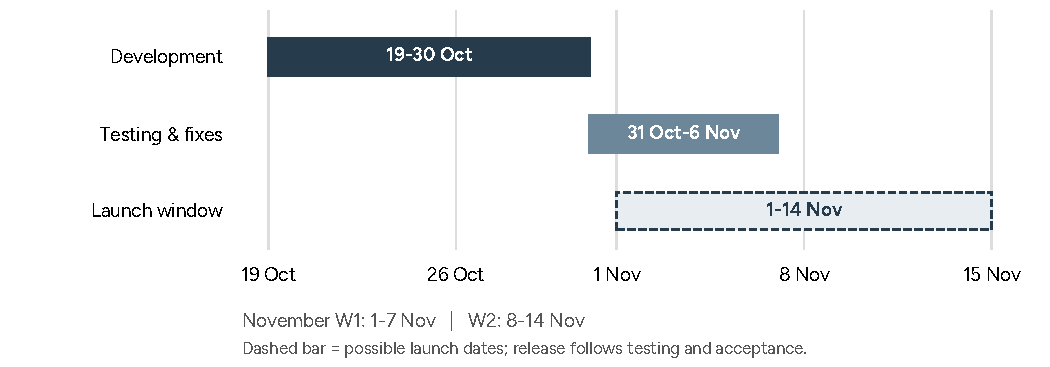
\includegraphics[width=\linewidth]{release-timeline.pdf}\end{center}

The earliest launch window overlaps testing: launch only after payment/\allowbreak{}wallet, enrollment/\allowbreak{}cancellation, payouts/\allowbreak{}referrals and access checks pass, release-blocking issues are resolved and the client accepts the release. Original report-branding assets, FAQ content and the agreed feature-video brief/\allowbreak{}materials should arrive during development; late materials or unresolved video scope may shift the affected deliverable or launch date. Review progress at the end of development to confirm the launch week.

\section*{References and review limits}

Primary source: FINAL SCOPE - Cogito Academy v3, October 12, 2026. Prior reference: October 11 Post-Meeting Scope and referral system.md. This revision incorporates October 13 client answers, project clarification on the friend cap, explicitly delegated implementation choices, and October 16 landing/\allowbreak{}report additions. The three-field report/\allowbreak{}in-app view exist in the reviewed repository; report PDF export remains planned. Production prices/\allowbreak{}live integrations have not been re-audited. This document does not change application behavior.
\clearpage
\input{RELEASE-V3-QUOTATION-BODY.tex}
\end{document}
